\documentclass[aspectratio=43]{beamer}

\usetheme{Padova}
\usepackage[utf8x]{inputenc}
\usepackage{listings}

\title{Progettazione e sviluppo di un'applicazione mobile per l'e-learning}
\author{Candidato: Marco Zanella \\Relatore:\hspace{13pt}Ombretta Gaggi \vspace{15pt}}
\date{21 settembre 2016}


\begin{document}
	
	\maketitle

	%\begin{frame}{Outline}
	%	\tableofcontents
	%\end{frame}


	%\section{Introduction}

	\begin{frame}{L'azienda ospitante}

		\begin{figure}[H]
			\centering
			
\includegraphics[scale=0.1]{images/logoMN}
		\end{figure}

	\end{frame}


	%\section{First section}

	\begin{frame}{Scopo dello stage}
		Progettare e sviluppare un'applicazione Android che deve permettere
		\begin{itemize}
			\item La fruizione dei corsi di e-learning sia online che offline
			\item Il download dei corsi nel dispositivo locale
			\item Il tracciamento di alcune azioni di interazione di un utente con un corso
		\end{itemize}
		%\begin{block}{Normal block}
		%	Fusce luctus venenatis felis quis semper
		%\end{block}

		%\begin{alertblock}{Alert block}
		%	$$ E = (x_1 \vee \neg x_2 \vee \neg x_3) \wedge (x_1 \vee x_2 \vee x_4) $$
		%\end{alertblock}

		%\begin{exampleblock}{Example block}
		%	Proin tincidunt, neque at tincidunt mollis
		%\end{exampleblock}
	\end{frame}

	\begin{frame}{Requisiti obbligatori}
		\begin{figure}[H]
			\centering
			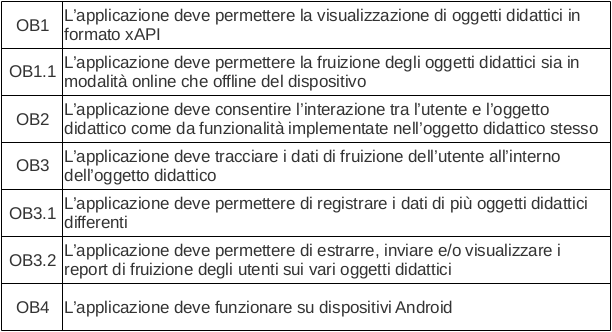
\includegraphics[scale=0.71]{images/obb}
		\end{figure}
	\end{frame}

	\begin{frame}{Requisiti opzionali}
		\begin{figure}[H]
			\centering
			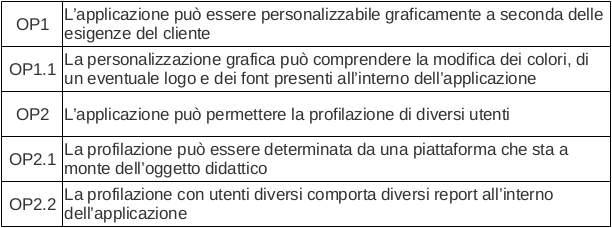
\includegraphics[scale=0.71]{images/opz}
		\end{figure}
	\end{frame}

	\begin{frame}{SCORM vs xAPI}
		Lo SCORM è lo standard de facto utilizzato per la creazione dei corsi di e-learning, ma non permette la fruizione offline. È possibile accedere ai corsi collegandosi ad un LMS tramite un browser\\
		\begin{figure}[H]
			\centering
			
\includegraphics[scale=0.5]{images/scorm}
		\end{figure}

		Nel 2013 però è stata creata la specifica xAPI(conosciuta anche come Experience API o Tin Can API)
		\begin{figure}[H]
			\centering
			
\includegraphics[scale=0.5]{images/tincanapi}
		\end{figure}
	\end{frame}

	\begin{frame}{La specifica xAPI}
		La specifica xAPI prevede
		\begin{itemize}
			\item Fruizione dei corsi all'esterno di browser e offline
			\item Tracciamento delle attività tramite statement
			\item Invio degli statement ad un LRS interno o esterno ad un LMS
		\end{itemize}
		Gli statement nella forma più semplice sono utilizzati per rappresentare frasi composte da soggetto verbo e complemento oggetto
	\end{frame}

	\begin{frame}[fragile]
	\frametitle{Esempio di statement}
\textit{``Mario Rossi ha iniziato il corso Corso di prova''}
\begin{lstlisting}[basicstyle=\tiny]
{
    "actor": {
        "objectType": "Agent",
        "name": "Mario Rossi",
        "mbox": "mailto:mariorossi@email.com"
    },
    "verb": {
        "id": "http://adlnet.gov/expapi/verbs/initialized",
        "display": {
            "en-US": "initialized"
        }
    },
    "object": {
        "objectType": "Activity",
        "id": "http://Corso%20di%20prova",
        "definition": {
            "description": {
                "und": "Corso di prova"
            },
            "type": "http://adlnet.gov/expapi/activities/module"
        }
    }
}
\end{lstlisting}
\end{frame}

	\begin{frame}{Analisi del progetto}
		Il primo periodo dello stage ha previsto
		\begin{itemize}
			\item Studio delle caratteristiche che il prodotto deve avere
			\item Ricerca e studio delle tecnologie più adatte
			\item Studio della specifica xAPI e ricerca di un LRS
			\item Ricerca di un metodo per recuperare i dati di fruizione di un utente
		\end{itemize}
	\end{frame}

	\begin{frame}{Progettazione e sviluppo}
		\begin{itemize}
			\item Impiego del pattern architetturale MVP unito all'utilizzo della dependency injection
			\item Creazione dello schema del database locale al dispositivo
			\item Codifica seguendo la strategia test driven development
		\end{itemize}
	\end{frame}

	\begin{frame}{Tecnologie utilizzate}
		%\begin{itemize}
		%	\item Android
		%	\item xAPI
		%	\item JavaScript
		%	\item Aggregation framework di MongoDB
		%\end{itemize}
		\begin{figure}[H]
			\centering
			
\includegraphics[scale=0.35]{images/tecnologie}
		\end{figure}
	\end{frame}

	\begin{frame}{Login e registrazione}
		\begin{figure}[H]
			\centering
			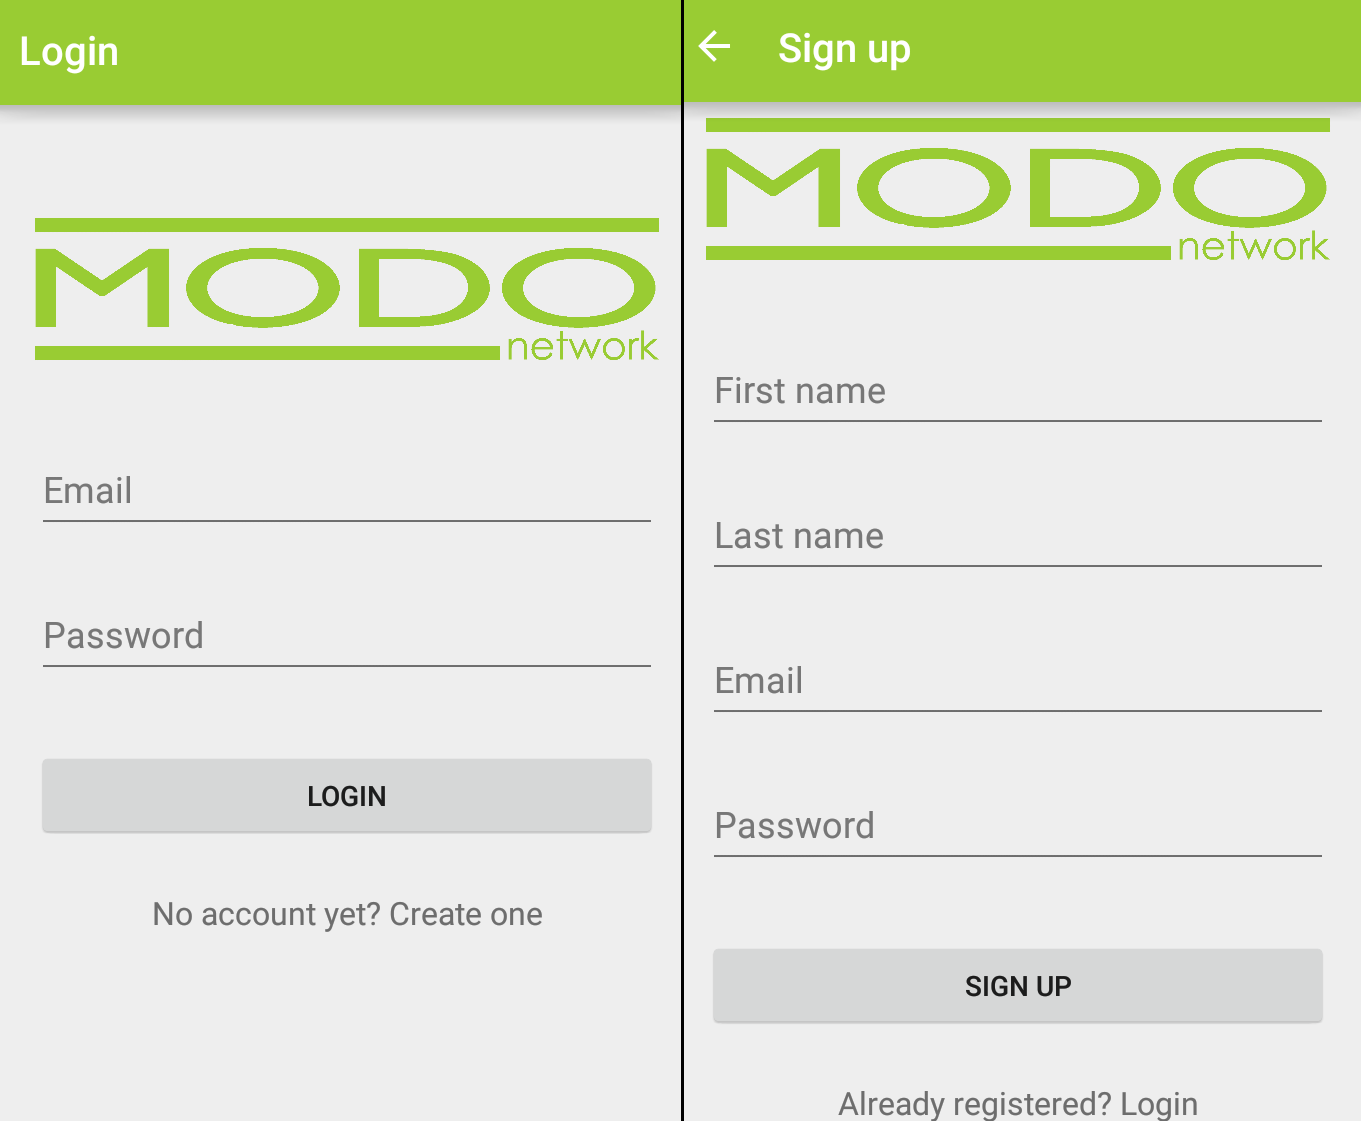
\includegraphics[scale=0.13]{images/prodotto_finale/loginSignUp}
		\end{figure}
	\end{frame}

	\begin{frame}{Home page}
		\begin{figure}[H]
			\centering
			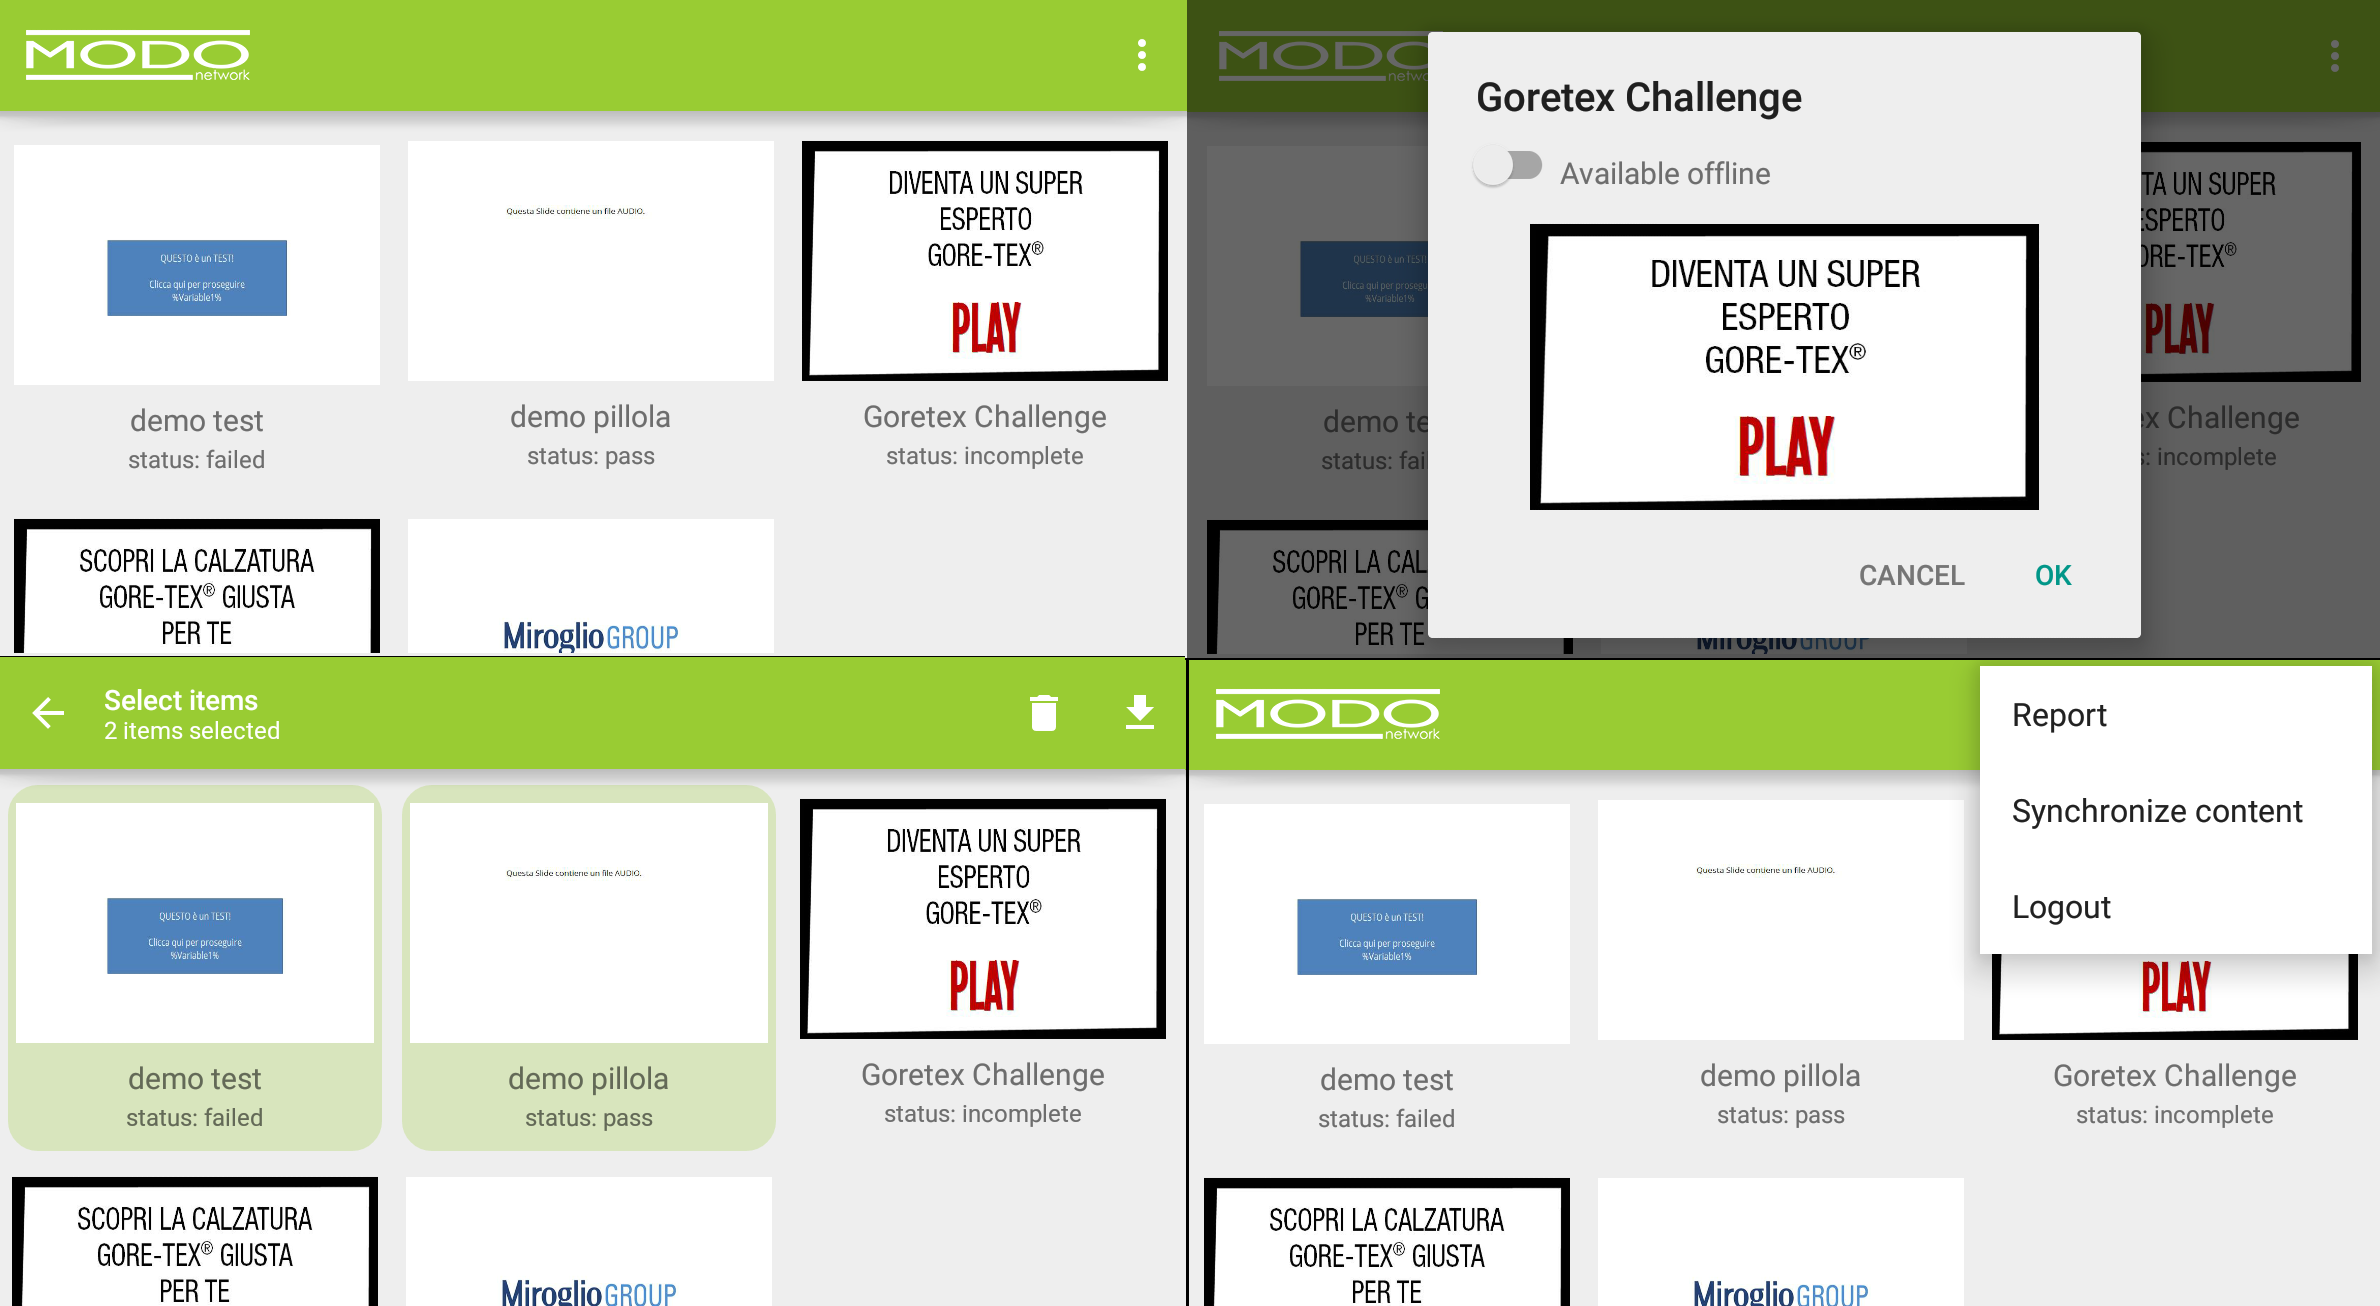
\includegraphics[scale=0.13]{images/prodotto_finale/homex4}
		\end{figure}
	\end{frame}

	\begin{frame}{Report}
		\begin{figure}[H]
			\centering
			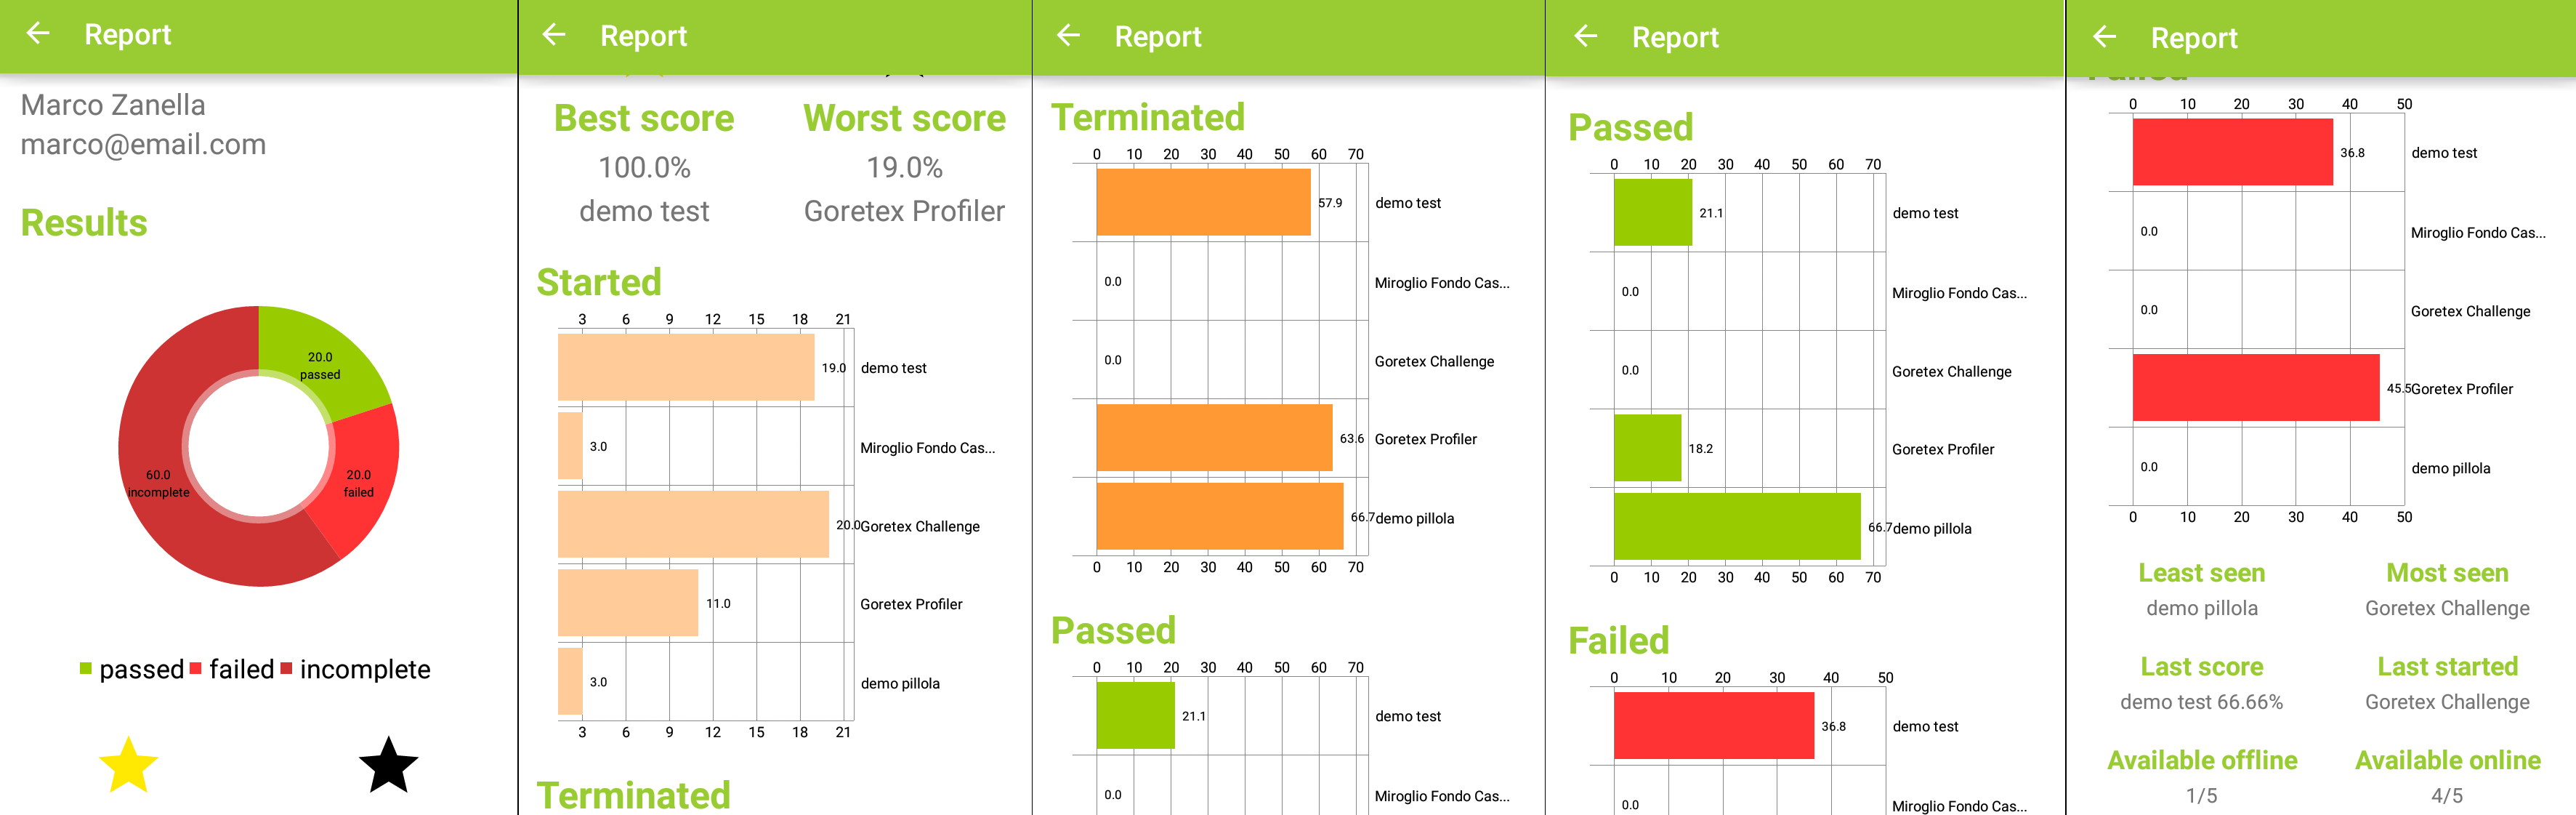
\includegraphics[scale=0.089]{images/prodotto_finale/report_tot}
		\end{figure}
	\end{frame}

	\begin{frame}{Fruizione dei contenuti}
		\begin{figure}[H]
			\centering
			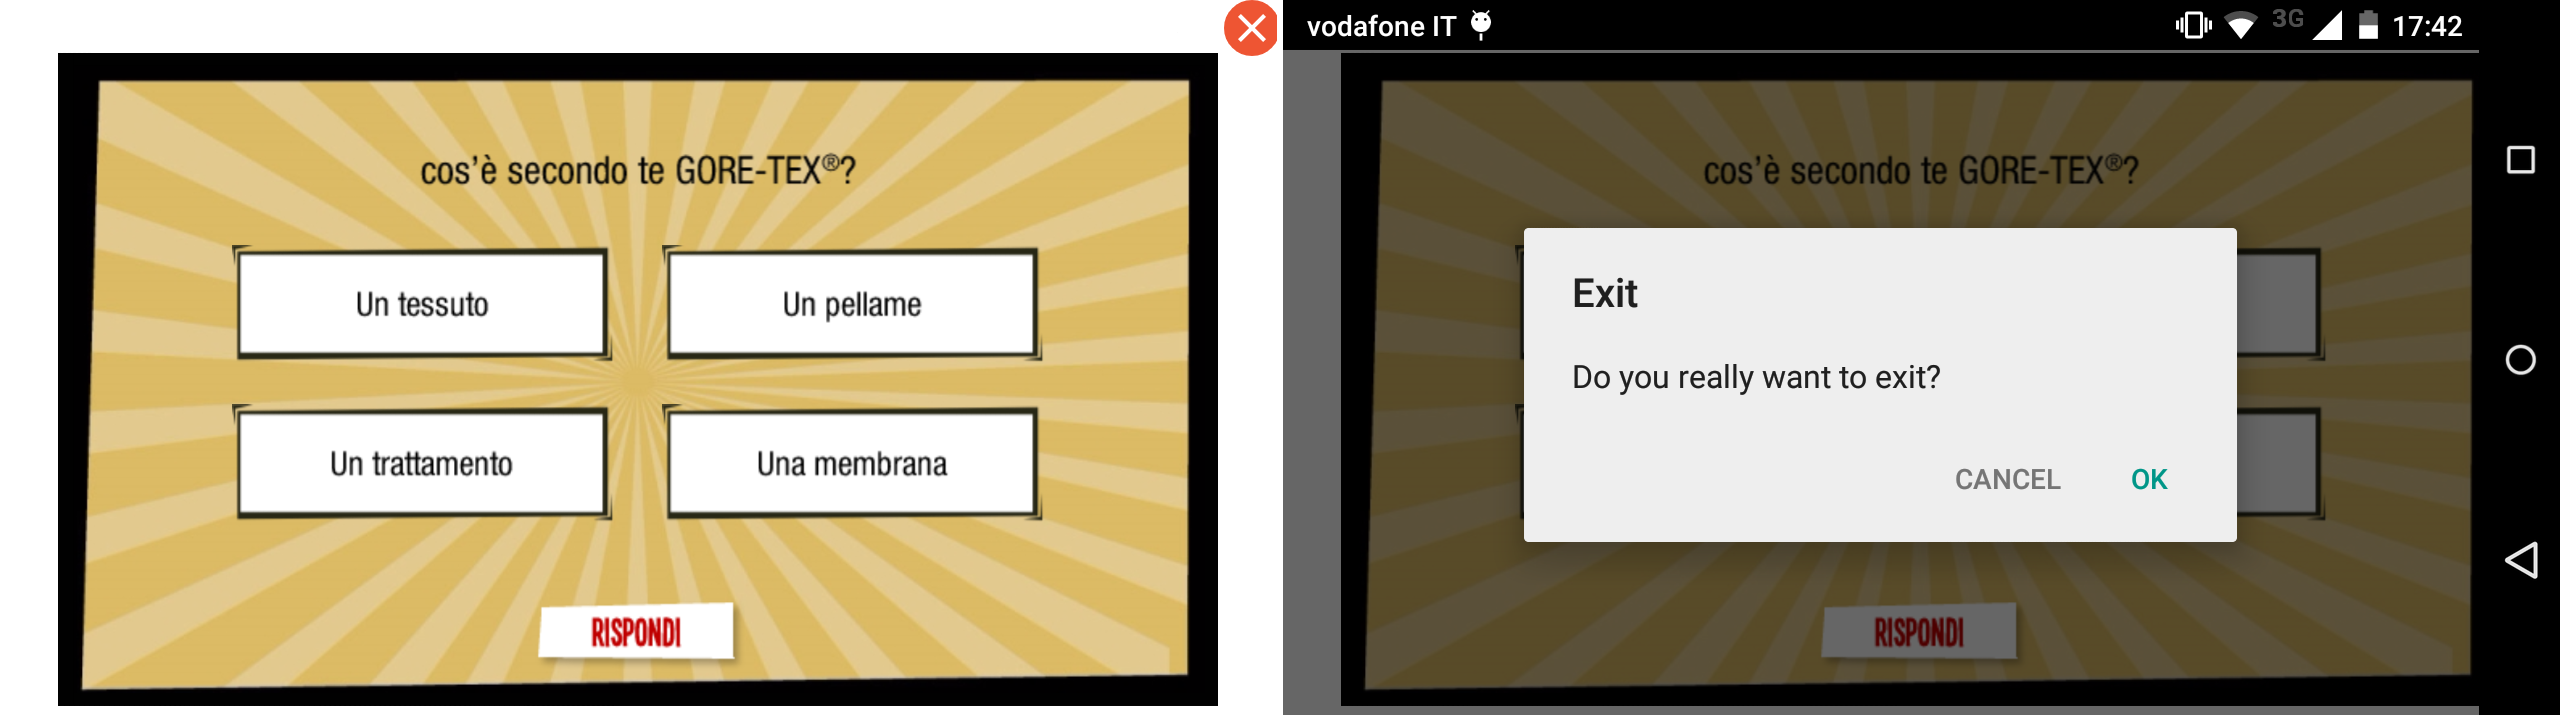
\includegraphics[scale=0.12]{images/prodotto_finale/content_tot}
		\end{figure}
	\end{frame}	

	\begin{frame}{Obiettivi raggiunti}
		\begin{figure}[H]
			\centering
			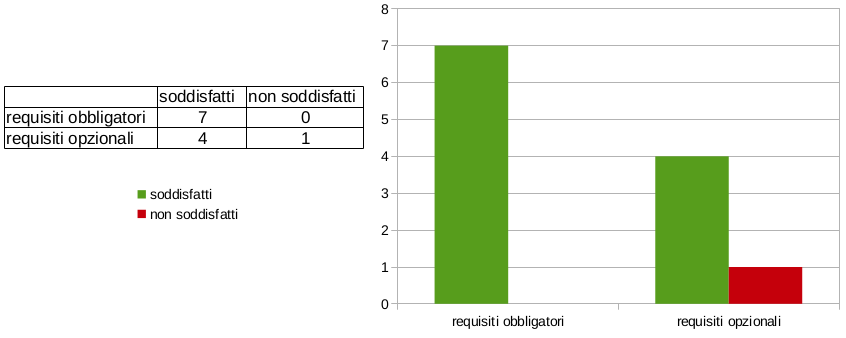
\includegraphics[scale=0.5]{images/requisiti}
		\end{figure}
	\end{frame}

	%\begin{frame}{Conclusioni}
	%	Lo stage ha presentato alcune problematiche
	%	\begin{itemize}
	%		\item Organizzazione del lavoro
	%		\item Rispetto delle scadenze
	%		\item Possibile integrazione con i social
	%		\item Creazione di un applicativo che si interfacci con l'LRS
	%	\end{itemize}
	%\end{frame}

	\begin{frame}{Sviluppi futuri}
		Alla fine dello stage l'applicazione presenta una serie di sviluppi futuri
		\begin{itemize}
			\item Creazione di un'applicazione per iOS
			\item Miglioramento del tracciamento delle attività di un utente
			\item Possibile integrazione con i social
			\item Creazione di un applicativo che si interfacci con l'LRS
		\end{itemize}
	\end{frame}

\end{document}
